\graphicspath{ {6-Experimento/} }

\chapter{Avaliação Experimental}

Como mencionado no Capítulo \ref{sgbd}, muitas empresas ainda utilizam 
bancos relacionais como forma de gerenciar seus dados. 
Por se tratar de um SGBD \textit{open source} e ser amplamente 
conhecido, foi escolhido para o estudo o PostgreSQL. Ele possui vasta 
documentação, tutoriais e suporte em fóruns sobre bancos de dados e 
programação de forma geral, além de receber recorrentes atualizações. 

O fato do PostgreSQL utilizar a Linguagem SQL como forma de 
manipulação de dados faz com que seja necessário também escolher 
o banco colunar para comparação utilizando esse filtro. Para tanto, o 
SGBDC escolhido foi o MonetDB, pioneiro na categoria colunar. A escolha também 
se deu com base na simplicidade do uso do SGBD, e na praticidade de 
migração dos dados armazenados entre um banco e outro. 

O gerenciamento dos SGBD foi realizado por meio do \textit{driver} JDBC 
disponibilizado nas páginas oficiais do PostgreSQL e do MonetDB. Seu uso se deu 
devido à simplificação no desenvolvimento de aplicações, por dar suporte a 
diferentes SGBD e possuir boa documentação e tutoriais. Na análise de tempo 
foi considerada a latência da Máquina Virtual Java (JVM), assim o tempo total 
das consultas corresponde ao tempo de execução pelo SGBD adicionado 
do tempo de resposta da JVM. As versões dos SGBD utilizadas 
foram o PostgreSQL 9.6 e o MonetDB 11.29.3 e foram instalados no servidor do laboratório GIA (Grupo de Pesquisa em Inteligência Aplicada), operando sob o 
sistema operacional Ubuntu Linux 16.04 LTS, com 16GB de RAM e dois 
processadores Intel Xeon CPU E5620 2.40GHz.

Os cenários de teste consistiram de três bases de dados de tamanhos 
diferentes, de 1GB, 10GB e 30GB para simular desde uma base pequena 
até bases maiores. Cada cenário foi executado nos ambientes \textit{snowflake} e 
\textit{star}.

Alguns fatores devem ser considerados ao executar testes de \textit{benchmark} 
no escopo de banco de dados \cite{raasveldt2018fair}:

\begin{enumerate}
    \item{O ambiente de execução 
    deve ser o mesmo para todos os SGBD, bem como a lógica e sequência de 
    execução.}
    \item{A modelagem do banco deve ser idêntica para todos os modelos, e isso 
    inclui os tipos de dados e restrições de integridade. Ao analisar os resultados do \textit{benchmark}, a menos 
    que seja especificado no estudo, não há como saber qual é o tipo de dado de um atributo 
    quando existem diferentes tipos que podem ser usados para a mesma função, 
    e essa diferença acarreta em resultados diferentes de desempenho. Por exemplo, 
    em Raasveldt et al. \cite{raasveldt2018fair} o SGBD MariaDB apresentou diferenças quando implementado 
    utilizando DECIMAL e DOUBLE.}
    \item{\textit{Cold run} vs. \textit{Hot run}: em alguns sistemas a primeira execução de 
    testes (\textit{cold}) costuma levar mais tempo para executar que as execuções subsequentes (\textit{hot}). 
    Isso se dá pelo buffer do banco de dados ou o próprio sistema operacional ter armazenado em 
    cache os dados requeridos.}
\end{enumerate}

\begin{figure*}[htpb]
	\centering
        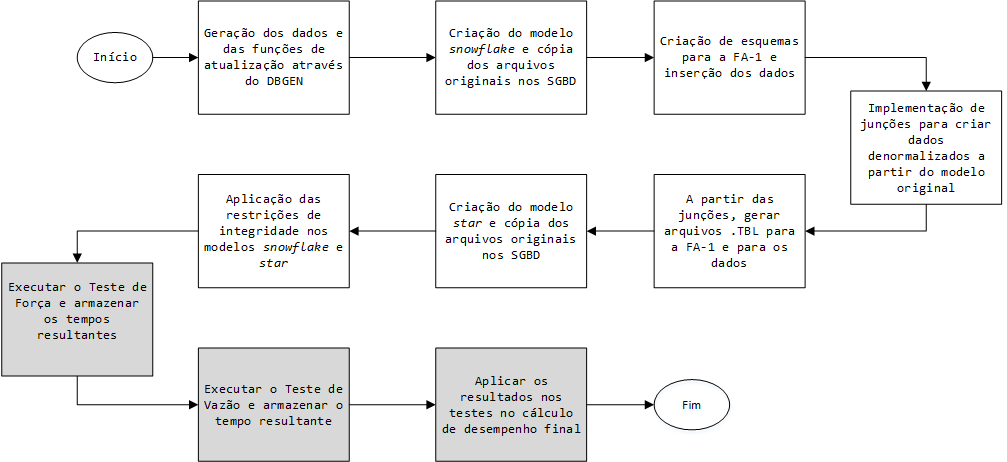
\includegraphics[width=\textwidth]{flux}
	\caption{Fluxograma do desenvolvimento até o cálculo final de desempenho do TPC-H}
	\label{fig:flux}
\end{figure*}

Os itens 1 e 2 foram tratados antes da execução do TPC-H. Nos Apêndices \ref{ddl_snow} e \ref{ddl_star} se encontram as SQL 
utilizadas para criar os esquemas \textit{snowflake} e \textit{star} nos SGBD. O fluxograma da Figura \ref{fig:flux} 
ilustra ainda a sequência de passos desde a criação dos bancos até a execução do \textit{benchmark}. 

O item 3 foi tratado durante a execução das consultas do teste de força: para cada cenário é realizada três 
análises diferentes, a primeira considerando a primeira execução de consultas; a segunda considerando o melhor 
resultado entre três execuções; e a terceira limpando parte da cache do sistema operacional antes de 
rodar a terceira execução. Essa análise é feita somente sob as consultas do teste de força por ser o primeiro 
teste a ser feito, como pode ser observado na Figura \ref{fig:power_flux}, que ilustra o fluxograma do teste de força. No teste de vazão todas as consultas já foram executadas 
uma vez e as funções de atualização trabalham sobre dados diferentes a cada vez que são executadas, impossibilitando 
o armazenamento em cache.

\begin{figure*}[htpb]
	\centering
        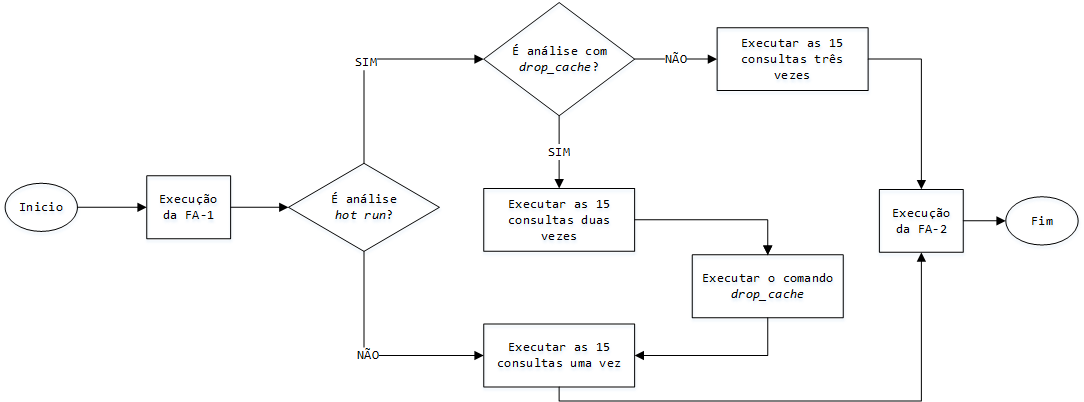
\includegraphics[width=\textwidth]{power_flux}
	\caption{Fluxograma do desenvolvimento do teste de força considerando todas as variações de cenário}
	\label{fig:power_flux}
\end{figure*}

Para averiguar se todas as 22 consultas do TPC-H executam de forma correta e em tempo hábil, principalmente 
atentando-se ao fato de que no ambiente denormalizado elas foram modificadas, foi realizada uma execução 
prévia de cada uma, sob a menor base de dados, utilizando o JDBC. Dessa execução, foram eliminadas as consultas 
Q2, Q4, Q15, Q17, Q20 e Q21 por terem demorado horas para executar -- e algumas tendo a execução 
cancelada antes -- enquanto que as demais levaram apenas alguns segundos para tal. As consultas Q2, Q15 e Q17 demoraram 
na modelagem denormalizada do PostgreSQL e a Q20 em sua modelagem normalizada; e as consultas Q4 e Q21 na modelagem denormalizada do MonetDB. A consulta 
Q1 também foi retirada do experimento por resultar em \textit{overflow} de cálculo na modelagem normalizada do MonetDB.

Essa mudança no número 
de consultas fez com que as equações originais fossem adaptadas para a nova quantidade, 15. Tem-se neste caso a 17ª raiz do produto dos termos no teste de força conforme a Equação \ref{eq:1-2}.

\begin{myequation}%
\label{eq:1-2}
{\scriptstyle Power@Size} = \frac{3600 * SF}{\sqrt[17]{\prod_{i = 1}^{i = 15}Q(i, 0) * \prod_{j = 1}^{j = 2}RF(j, 0)}} %
\end{myequation}
%

\begin{myequation}%
\label{eq:2-2}
{\scriptstyle Throughput@Size} = \frac{S * 15 * 3600}{T_s * SF} %
\end{myequation}
%

\section{Carregamento de Dados}

Após gerar todos os arquivos contendo os registros para inserção nos SGBD, foi utilizando o comando \textit{COPY}. Para se obter um melhor desempenho na inserção de dados as restrições de chaves foram aplicadas após a inserção de todos os dados. Caso a restrição fosse feita na criação do banco a cada novo registro inserido a chave primária seria verificada. Esta carga de dados também foi realizada através dos SGBD de forma direta, sem o uso de \textit{drivers} e outras ferramentas que possam atuar como cliente para conectar-se ao banco, assim evitando incluir o tempo de latência destas no resultado. Os comandos no MonetDB e no PostgreSQL são, respectivamente:

\begin{verbatim}
COPY INTO tabela FROM arquivo USING DELIMITERS delimitadores;
COPY tabela FROM arquivo DELIMITER delimitadores;
\end{verbatim}

A Tabela \ref{tab:carregamento} mostra o tempo em segundos para a inserção de dados nos SGBD. Logo ao analisar os resultados de carregamento de dados nota-se que um banco denormalizado apresenta certa demora na inserção de dados em relação a um normalizado. Isso se dá por causa da redundância de dados existente neste tipo de modelo, fazendo com que existam mais atributos duplicados em uma mesma entidade; aumentando o tamanho das entidades a serem inseridas. 

\begin{table}[htpb]
        \centering
        \caption{Tempo de carregamento em segundos para os cenários de \textit{benchmark}}
        \label{tab:carregamento}
        \begin{tabular}{c|ccc|c}
        \hline
        \multirow{2}{*}{SGBD} & \multicolumn{3}{c|}{Base de Dados (GB)} & \multirow{2}{*}{Ambiente}  \\
                              & 1           & 10          & 30          &                            \\ \hline
        MonetDB               & 44          & 409         & 1351        & \multirow{2}{*}{\textit{Snowflake}} \\
        PostgreSQL            & 104         & 816         & 4979        &                            \\ \hline
        MonetDB               & 88          & 689         & 2216        & \multirow{2}{*}{\textit{Star}}      \\
        PostgreSQL            & 166         & 2365        & 7216        &                            \\ \hline
        \end{tabular}
    \end{table}

Toma-se como exemplo a entidade \textit{nation}: no modelo \textit{snowflake} ela é uma tabela subdimensão e possui 25 registros apenas, enquanto que no modelo denormalizado ela faz parte das tabelas dimensão \textit{supplier} e \textit{customer}, fazendo com que estas duas entidades tenham mais bytes armazenados. A Tabela \ref{tab:tamanho} mostra o tamanho dos arquivos gerados para cada modelo para a base de dados de 1GB. Note que \textit{part} não tem seu valor alterado por não sofrer alteração entre as modelagens.

\begin{table}[htpb]
        \centering
        \caption{Tamanho em bytes das entidades}
        \label{tab:tamanho}
        \begin{tabular}{l|l|c|}
        \cline{2-3}
                                                     & \textit{Snowflake} & \textit{Star} \\ \hline
        \multicolumn{1}{|l|}{\textit{Supplier}}      & 1.409.184          & 2.990.430     \\ \hline
        \multicolumn{1}{|l|}{\textit{Customer}}      & 24.346.144         & 48.055.517    \\ \hline
        \multicolumn{1}{|l|}{\textit{Part}}          & 24.135.125         & 24.135.125    \\ \hline
        \multicolumn{1}{|l|}{\textit{Lineitem/Item}} & 759.863.287        & 2.226.620.122 \\ \hline
        \end{tabular}
        \end{table}


Um ponto importante a ser analisado foi o tamanho final de cada SGBD. A Tabela \ref{tab:carregamento_size} 
mostra que mesmo para a mesma quantidade de dados o MonetDB tem o tamanho em bytes reduzido, mostrando a capacidade 
que um SGBD colunar tem de realizar compressão de dados de forma mais eficiente.

\begin{table}[htpb]
    \centering
    \caption{Tamanho da base de dados nos SGBD em Mb para os cenários de \textit{benchmark}}
    \label{tab:carregamento_size}
    \begin{tabular}{c|ccc|c}
        \hline
        \multirow{2}{*}{SGBD} & \multicolumn{3}{c|}{Base de Dados (GB)} & \multirow{2}{*}{Ambiente}  \\
                              & 1           & 10          & 30          &                            \\ \hline
        MonetDB               & 771         & 8087        & 21352       & \multirow{2}{*}{\textit{Snowflake}} \\
        PostgreSQL            & 1567        & 15510       & 44371       &                            \\ \hline
        MonetDB               & 952         & 9352        & 26271       & \multirow{2}{*}{\textit{Star}}      \\
        PostgreSQL            & 2565        & 25487       & 71586       &                            \\ \hline
        \end{tabular}
    \end{table}

% -----------------------------
% COLD RUN

\section{Execução \textit{Cold Run}}

O primeiro cenário de execução consiste em analisar os resultados de desempenho considerando a primeira execução sequencial de todas as consultas do teste de força. 

\subsection{Base de Dados de 1GB}

Considerando fator de escala de 1GB, o número de registros das tabelas \textit{supplier, customer, part, partsupp, orders} e \textit{lineitem} são, respectivamente, 10.000, 150.000, 200.000, 800.000, 1.500.000 e 6.001.215. O número de registros das tabelas \textit{region} e \textit{nation} são fixos em 5 e 25, respectivamente. Também, em \textit{lineitem} o número de registros depende de um pedido em \textit{orders}, sendo definido sob um número aleatório entre um e quatro.

O primeiro conjunto de resultados para a execução de 1GB pode ser visto nas Tabelas \ref{tab:queries_cold_1} e \ref{tab:forca_vazao_cold_1}. A primeira mostra os tempos em segundos que os dois SGBD levaram para executar as RF e as 15 consultas. Nela é possível verificar que a primeira consulta (Q3) é a que mais consome tempo de execução, e que o MonetDB não tem desempenho melhor que o PostgreSQL na remoção de registros no ambiente \textit{snowflake}, e ao contrário do que se esperava, este SGBD em ambiente denormalizado levou mais tempo para processar as consultas ao normalizado. 

\begin{table}[htpb]
        \centering
        \caption{Tempo em segundos de todas as consultas do teste de força e funções de atualização sob \textit{cold run} para 1GB}
        \label{tab:queries_cold_1}
        \begin{tabular}{|c|c|c|c|c|} 
        \cline{2-5}
        \multicolumn{1}{c|}{} & \multicolumn{2}{c|}{\textit{\textbf{Snowflake}} } & \multicolumn{2}{c|}{\textit{\textbf{Star}} }  \\ 
        \hline
         \textbf{SGBD}        & \textbf{MonetDB}  & \textbf{PostgreSQL}           & \textbf{MonetDB}  & \textbf{PostgreSQL}       \\ 
        \hline
         \textbf{RF-1}        & 2.742             & 49.125                        & 2.975             & 45.889                    \\ 
        \hline
         \textbf{Q3}          & 9.094             & 13.615                        & 18.056            & 65.649                    \\ 
        \hline
         \textbf{Q5}          & 0.985             & 2.673                         & 1.877             & 3.851                     \\ 
        \hline
         \textbf{Q6}          & 1.846             & 3.365                         & 2.053             & 2.779                     \\ 
        \hline
         \textbf{Q7}          & 0.892             & 1.648                         & 1.324             & 2.913                     \\ 
        \hline
         \textbf{Q8}          & 1.256             & 2.685                         & 2.341             & 5.132                     \\ 
        \hline
         \textbf{Q9}          & 3.485             & 5.870                         & 3.867             & 5.375                     \\ 
        \hline
         \textbf{Q10}         & 0.983             & 2.975                         & 1.468             & 3.427                     \\ 
        \hline
         \textbf{Q11}         & 0.356             & 0.503                         & 2.224             & 7.608                     \\ 
        \hline
         \textbf{Q12}         & 2.199             & 2.958                         & 2.853             & 3.097                     \\ 
        \hline
         \textbf{Q13}         & 2.502             & 2.639                         & 11.019            & 12.157                    \\ 
        \hline
         \textbf{Q14}         & 0.129             & 2.012                         & 0.266             & 2.691                     \\ 
        \hline
         \textbf{Q16}         & 0.617             & 1.626                         & 1.766             & 9.761                     \\ 
        \hline
         \textbf{Q18}         & 1.613             & 6.968                         & 1.280             & 15.757                    \\ 
        \hline
         \textbf{Q19}         & 0.646             & 2.578                         & 0.922             & 3.508                     \\ 
        \hline
         \textbf{Q22}         & 0.323             & 0.979                         & 0.967             & 4.738                     \\ 
        \hline
         \textbf{Total}       & 26.925            & 53.092                        & 52.285            & 148.443                   \\ 
        \hline
         \textbf{RF-2}        & 40.812            & 38.091                        & 20.260            & 20.575                    \\
        \hline
        \end{tabular}
\end{table}

\begin{table}[htpb]
        \centering
        \caption{Valores do teste de força e vazão sob \textit{cold run} para 1GB}
        \label{tab:forca_vazao_cold_1}
        \begin{tabular}{|c|c|c|c|c|} 
        \cline{2-5}
        \multicolumn{1}{c|}{} & \multicolumn{2}{c|}{\textbf{Teste de Força} } & \multicolumn{2}{c|}{\textbf{Teste de Vazão} }  \\ 
        \hline
                \textbf{SGBD}        & \textbf{MonetDB}  & \textbf{PostgreSQL}       & \textbf{MonetDB}  & \textbf{PostgreSQL}        \\ 
        \hline
                \textbf{Snowflake}   & 2541.636          & 980.630                   & 1622.929          & 958.028                    \\ 
        \hline
                \textbf{Star}        & 1504.254          & 501.254                   & 2468.020          & 637.310                    \\
        \hline
        \end{tabular}
\end{table}

Na Tabela \ref{tab:forca_vazao_cold_1} é possível perceber que o SGBD que obteve resultados dentro do esperado foi o PostgreSQL. O desempenho considerando um único usuário ativo foi melhor no ambiente normalizado, assim como no teste simulando vários usuários ativos. O MonetDB só alcançou resultados melhores no ambiente denormalizado para o último teste.


% ---------------------------------
% BASE DE 10 GB

\subsection{Base de Dados de 10GB}

O número de registros das tabelas \textit{supplier, customer, part, partsupp} e \textit{orders} correspondem aos valores da base de 1GB, porém 10 vezes maior -- exceto \textit{lineitem}, cujo valor é 59.986.052. São, respectivamente, 100.000, 1.500.000, 2.000.000, 8.000.000, 15.000.000.

Nesta execução fica evidente a diferença de tempo da primeira consulta para as demais no SGBD colunar. Tomando a segunda mais lenta no MonetDB normalizado e denormalizado (Q13), a Q3 é 6.3 vezes no primeiro ambiente, e quase quatro vezes no segundo, mais demorada. Ainda, o ambiente denormalizado continua tendo desempenho pior que o normalizado no MonetDB, como é possível verificar na Tabela \ref{tab:queries_cold_10}. A Tabela \ref{tab:forca_vazao_cold_10} continua apresentando a mesma lógica que a Tabela \ref{tab:forca_vazao_cold_1} nos resultados.

\begin{table}[t]
        \centering
        \caption{Tempo em segundos de todas as consultas do teste de força e funções de atualização sob \textit{cold run} para 10GB}
        \label{tab:queries_cold_10}
        \begin{tabular}{|c|c|c|c|c|} 
                \cline{2-5}
                \multicolumn{1}{c|}{} & \multicolumn{2}{c|}{\textit{\textbf{Snowflake}} } & \multicolumn{2}{c|}{\textit{\textbf{Star}} }  \\ 
                \hline
                 \textbf{SGBD}        & \textbf{MonetDB}  & \textbf{PostgreSQL}           & \textbf{MonetDB}  & \textbf{PostgreSQL}       \\ 
                \hline
                 \textbf{RF-1}        & 14.351            & 1304.641                      & 12.596            & 1042.060                  \\ 
                \hline
                 \textbf{Q3}          & 125.044           & 108.010                       & 164.697           & 194.322                   \\ 
                \hline
                 \textbf{Q5}          & 8.762             & 37.100                        & 10.069            & 192.718                   \\ 
                \hline
                 \textbf{Q6}          & 18.130            & 19.793                        & 13.621            & 155.163                   \\ 
                \hline
                 \textbf{Q7}          & 2.913             & 28.333                        & 0.327             & 151.504                   \\ 
                \hline
                 \textbf{Q8}          & 9.072             & 25.755                        & 9.396             & 151.010                   \\ 
                \hline
                 \textbf{Q9}          & 18.126            & 93.686                        & 14.613            & 209.017                   \\ 
                \hline
                 \textbf{Q10}         & 5.551             & 46.611                        & 5.347             & 137.693                   \\ 
                \hline
                 \textbf{Q11}         & 3.416             & 10.951                        & 15.150            & 261.915                   \\ 
                \hline
                 \textbf{Q12}         & 15.206            & 29.331                        & 20.039            & 129.920                   \\ 
                \hline
                 \textbf{Q13}         & 19.837            & 35.913                        & 43.488            & 256.449                   \\ 
                \hline
                 \textbf{Q14}         & 0.443             & 19.775                        & 2.696             & 132.184                   \\ 
                \hline
                 \textbf{Q16}         & 4.251             & 14.154                        & 14.163            & 225.790                   \\ 
                \hline
                 \textbf{Q18}         & 8.330             & 137.693                       & 8.901             & 349.738                   \\ 
                \hline
                 \textbf{Q19}         & 4.347             & 25.855                        & 2.962             & 134.205                   \\ 
                \hline
                 \textbf{Q22}         & 2.367             & 14.979                        & 8.144             & 234.272                   \\ 
                \hline
                 \textbf{Total}       & 245.795           & 647.938                       & 333.613           & 2915.899                  \\ 
                \hline
                 \textbf{RF-2}        & 526.547           & 379.049                       & 157.183           & 196.822                   \\
                \hline
                \end{tabular}
                \end{table}

\begin{table}[htpb]
        \centering
        \caption{Valores do teste de força e vazão sob \textit{cold run} para 10GB}
        \label{tab:forca_vazao_cold_10}
        \begin{tabular}{|c|c|c|c|c|} 
                \cline{2-5}
                \multicolumn{1}{c|}{} & \multicolumn{2}{c|}{\textbf{Teste de Força} } & \multicolumn{2}{c|}{\textbf{Teste de Vazão} }  \\ 
                \hline
                        \textbf{SGBD}        & \textbf{MonetDB}  & \textbf{PostgreSQL}       & \textbf{MonetDB}  & \textbf{PostgreSQL}        \\ 
                \hline
                        \textbf{Snowflake}   & 3687.621          & 775.652                   & 330.479           & 364.541                    \\ 
                \hline
                        \textbf{Star}        & 3116.068          & 174.381                   & 583.560           & 149.455                    \\
                \hline
                \end{tabular}
                \end{table}
                
\subsection{Base de Dados de 30GB}

O número de registros das tabelas \textit{supplier, customer, part, partsupp} e \textit{orders} correspondem aos valores da base de 1GB, porém 30 vezes maior. São, respectivamente, 300.000, 4.500.000, 6.000.000, 24.000.000, 45.000.000, e \textit{lineitem} tem agora 179.998.372 registros.

Pela Tabela \ref{tab:queries_cold_30} pode-se verificar que no SGBD colunar o comportamento permanece o mesmo às bases anteriores. Desta vez ainda a escalabilidade do tempo da consulta Q14 aumentou em 208 vezes em comparação à base de 1GB no ambiente normalizado e 334 vezes no denormalizado, enquanto que as demais consultas escalaram em um intervalo de valores com menos discrepâncias, ficando entre 13 e 75, e 12 e 69. Os resultados do teste de força e vazão são apresentados na Tabela \ref{tab:forca_vazao_cold_30}.

\begin{table}[t]
        \centering
        \caption{Tempo em segundos de todas as consultas do teste de força e funções de atualização sob \textit{cold run} para 30GB}
        \label{tab:queries_cold_30}
        \begin{tabular}{|c|c|c|c|c|} 
                \cline{2-5}
                \multicolumn{1}{c|}{} & \multicolumn{2}{c|}{\textit{\textbf{Snowflake}} } & \multicolumn{2}{c|}{\textit{\textbf{Star}} }  \\ 
                \hline
                 \textbf{SGBD}        & \textbf{MonetDB}  & \textbf{PostgreSQL}           & \textbf{MonetDB}  & \textbf{PostgreSQL}       \\ 
                \hline
                 \textbf{RF-1}        & 45.464            & 4346.899                      & 29.397            & 4011.410                  \\ 
                \hline
                 \textbf{Q3}          & 250.579           & 369.306                       & 507.637           & 566.055                   \\ 
                \hline
                 \textbf{Q5}          & 43.135            & 415.032                       & 79.365            & 581.650                   \\ 
                \hline
                 \textbf{Q6}          & 87.109            & 203.049                       & 70.875            & 525.149                   \\ 
                \hline
                 \textbf{Q7}          & 12.287            & 302.879                       & 24.758            & 542.459                   \\ 
                \hline
                 \textbf{Q8}          & 24.375            & 286.555                       & 45.394            & 545.627                   \\ 
                \hline
                 \textbf{Q9}          & 104.949           & 597.415                       & 54.817            & 717.576                   \\ 
                \hline
                 \textbf{Q10}         & 14.495            & 296.734                       & 19.087            & 545.421                   \\ 
                \hline
                 \textbf{Q11}         & 9.308             & 50.995                        & 68.687            & 1073.476                  \\ 
                \hline
                 \textbf{Q12}         & 96.438            & 260.277                       & 79.686            & 531.999                   \\ 
                \hline
                 \textbf{Q13}         & 62.886            & 124.179                       & 194.227           & 937.462                   \\ 
                \hline
                 \textbf{Q14}         & 26.823            & 219.780                       & 89.018            & 549.628                   \\ 
                \hline
                 \textbf{Q16}         & 11.826            & 74.054                        & 68.930            & 834.195                   \\ 
                \hline
                 \textbf{Q18}         & 109.423           & 796.233                       & 88.697            & 1225.532                  \\ 
                \hline
                 \textbf{Q19}         & 48.729            & 191.799                       & 46.524            & 482.566                   \\ 
                \hline
                 \textbf{Q22}         & 8.121             & 88.714                        & 25.656            & 969.976                   \\ 
                \hline
                 \textbf{Total}       & 910.485           & 4277.000                      & 1463.358          & 10628.772                 \\ 
                \hline
                 \textbf{RF-2}        & 1392.401          & 1120.928                      & 735.083           & 586.293                   \\
                \hline
                \end{tabular}
                \end{table}

\begin{table}[htpb]
        \centering
        \caption{Valores do teste de força e vazão sob \textit{cold run} para 30GB}
        \label{tab:forca_vazao_cold_30}
        \begin{tabular}{|c|c|c|c|c|} 
                \cline{2-5}
                \multicolumn{1}{c|}{} & \multicolumn{2}{c|}{\textbf{Teste de Força} } & \multicolumn{2}{c|}{\textbf{Teste de Vazão} }  \\ 
                \hline
                 \textbf{SGBD}        & \textbf{MonetDB}  & \textbf{PostgreSQL}       & \textbf{MonetDB}  & \textbf{PostgreSQL}        \\ 
                \hline
                 \textbf{Snowflake}   & 2329.918          & 369.019                   & 112.572           & 220.005                    \\ 
                \hline
                 \textbf{Star}        & 1474.766          & 145.064                   & 165.419           & 120.578                    \\
                \hline
                \end{tabular}
                \end{table}

\subsection{Desempenho Geral}

No cenário rodando sob \textit{cold run} o MonetDB não obteve resultados considerados estáveis como o PostgreSQL. Embora haja a conclusão que o SGBD colunar é melhor que o relacional, avaliando os dados dentro do MonetDB não se sabe qual modelagem é melhor devido à inflexão na base de dados de 10GB, trazendo incerteza na sua escolha. 

Considerando vários usuários ativos o resultado foi como esperado. Se considerar também somente as RF, o MonetDB teve valores muito superiores para inserção de dados, e na remoção somente para uma base de dados maior no ambiente denormalizado o PostgreSQL foi melhor. O que impactou nos resultados do SGBD colunar foi o comportamento anormal das consultas, onde a primeira demora um tempo excessivo para ser processada, enquanto as demais não e ainda não se segue uma lógica de escalabilidade no tempo conforme a base de dados aumenta.

O comportamento do teste de força no banco MonetDB não segue uma queda conforme a base de dados aumenta. Existe uma inflexão na base de dados de 10GB, pois não há um comportamento similar entre as consultas como acontece no PostgreSQL. Os gráficos das Figuras \ref{fig:power_snow_cold} e \ref{fig:power_star_cold} evidenciam isso. 

\begin{figure*}[htpb]
        \centering
        \subfigure[]{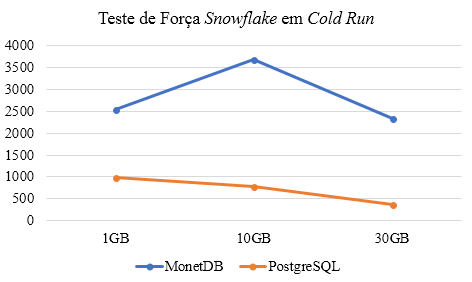
\includegraphics[width=7.2cm]{power_snow_cold}\label{fig:power_snow_cold}}
        \subfigure[]{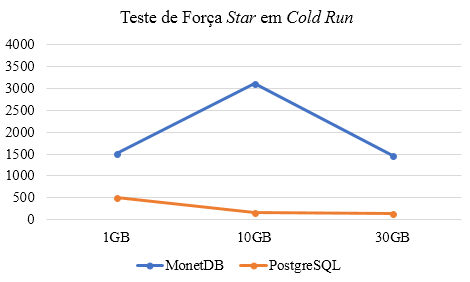
\includegraphics[width=7.2cm]{power_star_cold}\label{fig:power_star_cold}}
        \caption{Gráficos de força entre ambientes sob \textit{cold run}}
        \label{fig:power_cold}
\end{figure*}

O cálculo de desempenho final foi afetado por essa inflexão. Se analisar os resultados considerando os SGBD sob as modelagens \textit{snowflake} e \textit{star}, o MonetDB se destaca no resultado final, fazendo dele a melhor escolha entre os SGBD, como mostram os gráficos da Figuras \ref{fig:qph_snow_cold} e \ref{fig:qph_star_cold} e os ganhos obtidos por ele em relação ao PostgreSQL conforme a Tabela \ref{tab:ganho_monet_psql_cold}. Porém ao considerar os ambientes sob cada SGBD, a única conclusão coerente que se tem é de que o PostgreSQL é melhor em ambientes normalizados, como ilustram os gráficos das Figuras \ref{fig:qph_monet_cold} e \ref{fig:qph_psql_cold}, no qual conforme a base de dados aumenta o cálculo de desempenho é menor e sempre há ganhos do normalizado em relação ao denormalizado, sendo estes \textbf{42\%, 70\%} e \textbf{54\%} para 1GB, 10GB e 30GB, respectivamente.

\begin{figure*}[htpb]
        \centering
        \subfigure[]{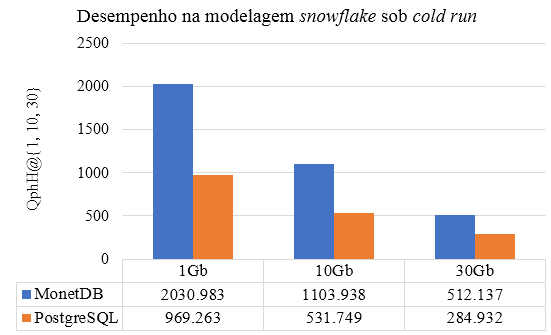
\includegraphics[width=7.2cm]{qph_snow_cold}\label{fig:qph_snow_cold}}
        \subfigure[]{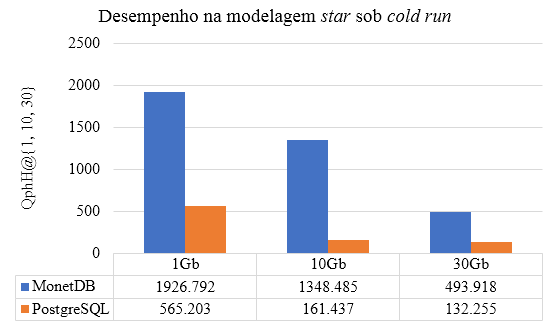
\includegraphics[width=7.2cm]{qph_star_cold}\label{fig:qph_star_cold}}
        \caption{Gráficos de desempenho entre ambientes sob \textit{cold run}}
        \label{fig:qph_model_cold}
\end{figure*}

\begin{table}[htpb]
        \centering
        \caption{Porcentagem de ganho de desempenho do MonetDB em relação ao PostgreSQL sob \textit{cold run}}
        \label{tab:ganho_monet_psql_cold}
        \begin{tabular}{|c|c|c|c|}
        \hline
        \multirow{2}{*}{\textbf{Ambiente}} & \multicolumn{3}{c|}{\textbf{Base de Dados (GB)}} \\ \cline{2-4} 
                                           & \textbf{1}     & \textbf{10}    & \textbf{30}    \\ \hline
        \textit{Snowflake}                 & 110\%          & 108\%          & 80\%           \\ \hline
        \textit{Star}                      & 241\%          & 735\%          & 273\%          \\ \hline
        \end{tabular}
\end{table}

\begin{figure*}[htpb]
        \centering
        \subfigure[]{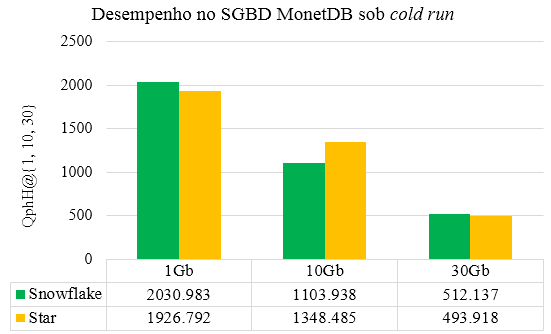
\includegraphics[width=7.2cm]{qph_monet_cold}\label{fig:qph_monet_cold}}
        \subfigure[]{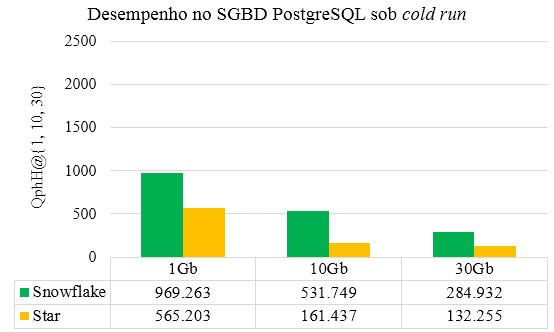
\includegraphics[width=7.2cm]{qph_psql_cold}\label{fig:qph_psql_cold}}
        \caption{Gráficos de desempenho entre SGBD sob \textit{cold run}}
        \label{fig:qph_sgbd_cold}
\end{figure*}

O MonetDB não segue uma lógica da qual se pode tirar alguma conclusão de acordo com a modelagem. Conforme o tamanho da base de dados aumenta o valor diminui assim como no PostgreSQL, porém entre as modelagens há uma inconsistência na comparação entre seus valores, visto que para 1GB o ambiente normalizado foi melhor com ganho de \textbf{5\%}, já para 10GB foi o denormalizado com \textbf{22\%} de ganho, e para 30GB o comportamento é como em 1GB com \textbf{4\%} de ganho do normalizado. 

% --------------------------------------------
% HOT RUN

\section{Execução \textit{Hot Run}}

O segundo cenário de execução analisa os resultados de desempenho considerando a terceira execução sequencial de todas as consultas do teste de força, sendo esta executada imediatamente após as duas primeiras. O objetivo é verificar se há diferença nos resultados encontrados no cenário anterior. Os registros e a quantidade são os mesmos dos cenários anteriores. 

\subsection{Base de Dados de 1GB}

Na terceira execução de todas as consultas já se nota uma grande diferença nos valores do MonetDB, tanto no ambiente normalizado quanto no denormalizado. A primeira consulta já não é a mais lenta, e todas as demais têm valores similares considerando que a base de dados é pequena, como mostra a Tabela \ref{tab:queries_hot_1}. Percebe-se também que agora o ambiente denormalizado não é mais lento que o normalizado. Este resultado impacta nos valores de força, visto que pode-se analisar a partir da Tabela \ref{tab:forca_vazao_hot_1} que agora o ambiente \textit{star} tem valor superior ao \textit{snowflake} no MonetDB. Não apenas superior, os valores resultantes do teste de força possuem magnitude maior que os do cenário anterior devido a eficiência do processamento das consultas.

% TABELA DE TEMPO DE CONSULTAS E RF
\begin{table}[t]
        \centering
        \caption{Tempo em segundos de todas as consultas do teste de força e funções de atualização sob \textit{hot run} para 1GB}
        \label{tab:queries_hot_1}
        \begin{tabular}{|c|c|c|c|c|} 
                \cline{2-5}
                \multicolumn{1}{c|}{} & \multicolumn{2}{c|}{\textit{\textbf{Snowflake}} } & \multicolumn{2}{c|}{\textit{\textbf{Star}} }  \\ 
                \hline
                 \textbf{SGBD}        & \textbf{MonetDB}  & \textbf{PostgreSQL}           & \textbf{MonetDB}  & \textbf{PostgreSQL}       \\ 
                \hline
                 \textbf{RF-1}        & 2.742             & 49.125                        & 2.975             & 45.889                    \\ 
                \hline
                 \textbf{Q3}          & 0.184             & 1.874                         & 0.079             & 3.231                     \\ 
                \hline
                 \textbf{Q5}          & 0.116             & 1.165                         & 0.063             & 3.303                     \\ 
                \hline
                 \textbf{Q6}          & 0.047             & 2.126                         & 0.051             & 2.762                     \\ 
                \hline
                 \textbf{Q7}          & 0.149             & 1.611                         & 0.067             & 2.796                     \\ 
                \hline
                 \textbf{Q8}          & 0.519             & 2.178                         & 0.078             & 3.344                     \\ 
                \hline
                 \textbf{Q9}          & 0.301             & 5.004                         & 0.089             & 5.187                     \\ 
                \hline
                 \textbf{Q10}         & 0.090             & 2.703                         & 0.049             & 3.381                     \\ 
                \hline
                 \textbf{Q11}         & 0.099             & 0.499                         & 0.102             & 7.510                     \\ 
                \hline
                 \textbf{Q12}         & 0.161             & 2.955                         & 0.070             & 3.085                     \\ 
                \hline
                 \textbf{Q13}         & 0.155             & 2.609                         & 0.092             & 12.106                    \\ 
                \hline
                 \textbf{Q14}         & 0.050             & 2.008                         & 0.060             & 2.593                     \\ 
                \hline
                 \textbf{Q16}         & 0.383             & 1.708                         & 0.667             & 9.359                     \\ 
                \hline
                 \textbf{Q18}         & 0.768             & 6.949                         & 0.508             & 8.970                     \\ 
                \hline
                 \textbf{Q19}         & 0.140             & 2.553                         & 0.121             & 3.204                     \\ 
                \hline
                 \textbf{Q22}         & 0.073             & 0.973                         & 0.090             & 3.777                     \\ 
                \hline
                 \textbf{Total}       & 3.236             & 36.918                        & 2.184             & 74.606                    \\ 
                \hline
                 \textbf{RF-2}        & 40.812            & 38.091                        & 20.260            & 20.575                    \\
                \hline
                \end{tabular}
\end{table}

% TABELA DE POWER E VAZÃO

\begin{table}[htpb]
        \centering
        \caption{Valores do teste de força e vazão sob \textit{hot run} para 1GB}
        \label{tab:forca_vazao_hot_1}
        \begin{tabular}{|c|c|c|c|c|} 
                \cline{2-5}
                \multicolumn{1}{c|}{}         & \multicolumn{2}{c|}{\textbf{Teste de Força} } & \multicolumn{2}{c|}{\textbf{Teste de Vazão} }  \\ 
                \hline
                 \textbf{SGBD}                & \textbf{MonetDB}  & \textbf{PostgreSQL}       & \textbf{MonetDB}  & \textbf{PostgreSQL}        \\ 
                \hline
                 \textit{\textbf{Snowflake}}  & 14043.395         & 1222.570                  & 1622.929          & 958.028                    \\ 
                \hline
                 \textit{\textbf{Star}}       & 21811.705         & 659.758                   & 2468.020          & 637.310                    \\
                \hline
                \end{tabular}
\end{table}


% ---------------------------------
% BASE DE 10 GB

\subsection{Base de Dados de 10GB}

Assim como a base de dados de 1GB, a de 10GB possui um comportamento que trazem resultados melhores que no cenário considerando \textit{cold run}, e novamente o MonetDB apresentou valores mais consistentes, e o ambiente denormalizado apresentou resultados melhores que o normalizado, como mostram as Tabelas \ref{tab:queries_hot_10} e \ref{tab:forca_vazao_hot_10}.

\begin{table}[t]
        \centering
        \caption{Tempo em segundos de todas as consultas do teste de força e funções de atualização sob \textit{hot run} para 10GB}
        \label{tab:queries_hot_10}
        \begin{tabular}{|c|c|c|c|c|} 
                \cline{2-5}
                \multicolumn{1}{c|}{} & \multicolumn{2}{c|}{\textit{\textbf{Snowflake}} } & \multicolumn{2}{c|}{\textit{\textbf{Star}} }  \\ 
                \hline
                 \textbf{SGBD}        & \textbf{MonetDB}  & \textbf{PostgreSQL}           & \textbf{MonetDB}  & \textbf{PostgreSQL}       \\ 
                \hline
                 \textbf{RF-1}        & 14.351            & 1304.641                      & 12.596            & 1042.060                  \\ 
                \hline
                 \textbf{Q3}          & 2.118             & 36.095                        & 1.506             & 125.089                   \\ 
                \hline
                 \textbf{Q5}          & 1.171             & 34.593                        & 1.273             & 159.875                   \\ 
                \hline
                 \textbf{Q6}          & 0.438             & 19.789                        & 0.602             & 132.427                   \\ 
                \hline
                 \textbf{Q7}          & 2.679             & 28.960                        & 1.277             & 146.097                   \\ 
                \hline
                 \textbf{Q8}          & 6.416             & 24.142                        & 1.428             & 126.529                   \\ 
                \hline
                 \textbf{Q9}          & 3.004             & 107.818                       & 0.597             & 170.805                   \\ 
                \hline
                 \textbf{Q10}         & 1.324             & 35.949                        & 0.223             & 128.092                   \\ 
                \hline
                 \textbf{Q11}         & 2.515             & 5.494                         & 0.686             & 263.927                   \\ 
                \hline
                 \textbf{Q12}         & 3.649             & 29.372                        & 1.505             & 122.578                   \\ 
                \hline
                 \textbf{Q13}         & 6.173             & 31.265                        & 8.303             & 261.873                   \\ 
                \hline
                 \textbf{Q14}         & 0.390             & 18.737                        & 0.161             & 132.393                   \\ 
                \hline
                 \textbf{Q16}         & 1.161             & 14.239                        & 6.757             & 225.479                   \\ 
                \hline
                 \textbf{Q18}         & 8.136             & 125.887                       & 5.643             & 339.079                   \\ 
                \hline
                 \textbf{Q19}         & 2.356             & 26.911                        & 1.801             & 125.114                   \\ 
                \hline
                 \textbf{Q22}         & 0.570             & 19.855                        & 2.736             & 215.812                   \\ 
                \hline
                 \textbf{Total}       & 42.100            & 559.107                       & 34.498            & 2675.167                  \\ 
                \hline
                 \textbf{RF-2}        & 526.547           & 379.049                       & 157.183           & 196.822                   \\
                \hline
                \end{tabular}
                \end{table}

\begin{table}[htpb]
        \centering
        \caption{Valores do teste de força e vazão sob \textit{hot run} para 10GB}
        \label{tab:forca_vazao_hot_10}
        \begin{tabular}{|c|c|c|c|c|} 
                \cline{2-5}
                \multicolumn{1}{c|}{}         & \multicolumn{2}{c|}{\textbf{Teste de Força} } & \multicolumn{2}{c|}{\textbf{Teste de Vazão} }  \\ 
                \hline
                 \textbf{SGBD}                & \textbf{MonetDB}  & \textbf{PostgreSQL}       & \textbf{MonetDB}  & \textbf{PostgreSQL}        \\ 
                \hline
                 \textit{\textbf{Snowflake}}  & 11861.997         & 870.994                   & 330.479           & 364.541                    \\ 
                \hline
                 \textit{\textbf{Star}}       & 17902.155         & 190.307                   & 583.560           & 149.455                    \\
                \hline
                \end{tabular}
                \end{table}

\subsection{Base de Dados de 30GB}

Para a base de 30GB além de manter-se o comportamento das anteriores, percebe-se um distanciamento maior dos valores do MonetDB para o PostgreSQL em \textit{hot run}. Os valores da Tabela \ref{tab:queries_hot_30} mostram isso e a Tabela \ref{tab:forca_vazao_hot_30} apresenta os valores de força e vazão.

\begin{table}[t]
        \centering
        \caption{Tempo em segundos de todas as consultas do teste de força e funções de atualização sob \textit{hot run} para 30GB}
        \label{tab:queries_hot_30}
        \begin{tabular}{|c|c|c|c|c|} 
                \cline{2-5}
                \multicolumn{1}{c|}{} & \multicolumn{2}{c|}{\textit{\textbf{Snowflake}} } & \multicolumn{2}{c|}{\textit{\textbf{Star}} }  \\ 
                \hline
                 \textbf{SGBD}        & \textbf{MonetDB}  & \textbf{PostgreSQL}           & \textbf{MonetDB}  & \textbf{PostgreSQL}       \\ 
                \hline
                 \textbf{RF-1}        & 45.464            & 4346.899                      & 29.397            & 4011.410                  \\ 
                \hline
                 \textbf{Q3}          & 68.066            & 329.075                       & 57.567            & 553.795                   \\ 
                \hline
                 \textbf{Q5}          & 12.812            & 373.031                       & 12.553            & 537.089                   \\ 
                \hline
                 \textbf{Q6}          & 2.579             & 186.510                       & 1.608             & 473.006                   \\ 
                \hline
                 \textbf{Q7}          & 3.086             & 279.495                       & 1.487             & 501.833                   \\ 
                \hline
                 \textbf{Q8}          & 6.984             & 281.131                       & 6.220             & 507.657                   \\ 
                \hline
                 \textbf{Q9}          & 60.413            & 607.088                       & 30.875            & 671.788                   \\ 
                \hline
                 \textbf{Q10}         & 11.154            & 310.681                       & 9.409             & 518.880                   \\ 
                \hline
                 \textbf{Q11}         & 9.597             & 68.390                        & 9.784             & 980.716                   \\ 
                \hline
                 \textbf{Q12}         & 42.212            & 261.946                       & 40.280            & 476.657                   \\ 
                \hline
                 \textbf{Q13}         & 62.234            & 144.715                       & 56.124            & 916.111                   \\ 
                \hline
                 \textbf{Q14}         & 1.576             & 224.288                       & 1.297             & 551.986                   \\ 
                \hline
                 \textbf{Q16}         & 11.634            & 75.528                        & 13.937            & 835.383                   \\ 
                \hline
                 \textbf{Q18}         & 56.660            & 771.133                       & 49.197            & 1224.231                  \\ 
                \hline
                 \textbf{Q19}         & 28.730            & 186.968                       & 27.263            & 495.281                   \\ 
                \hline
                 \textbf{Q22}         & 7.037             & 104.941                       & 6.001             & 1127.978                  \\ 
                \hline
                 \textbf{Total}       & 384.775           & 4204.921                      & 323.601           & 10372.392                 \\ 
                \hline
                 \textbf{RF-2}        & 1392.401          & 1120.928                      & 735.083           & 586.293                   \\
                \hline
                \end{tabular}
                \end{table}

\begin{table}[htpb]
        \centering
        \caption{Valores do teste de força e vazão sob \textit{hot run} para 30GB}
        \label{tab:forca_vazao_hot_30}
        \begin{tabular}{|c|c|c|c|c|} 
                \cline{2-5}
                \multicolumn{1}{c|}{}         & \multicolumn{2}{c|}{\textbf{Teste de Força} } & \multicolumn{2}{c|}{\textbf{Teste de Vazão} }  \\ 
                \hline
                        \textbf{SGBD}                & \textbf{MonetDB}  & \textbf{PostgreSQL}       & \textbf{MonetDB}  & \textbf{PostgreSQL}        \\ 
                \hline
                        \textit{\textbf{Snowflake}}  & 5457.325          & 363.441                   & 112.572           & 220.005                    \\ 
                \hline
                        \textit{\textbf{Star}}       & 6873.122          & 149.514                   & 165.419           & 120.578                    \\
                \hline
                \end{tabular}
                \end{table}
\subsection{Desempenho Geral}

Ao contrário do cenário sob \textit{cold run}, utilizar o terceiro conjunto de consultas trouxe estabilidade nos valores das consultas do teste de força no MonetDB. Isso fez com que a inflexão que antes acontecia não acontecesse mais, podendo agora encontrar uma lógica na análise dos ambientes considerando o SGBD. As Figuras \ref{fig:power_snow_hot} e \ref{fig:power_star_hot} apresentam os gráficos do teste de força, agora apresentando queda nos valores conforme a base de dados aumenta.

\begin{figure*}[t]
        \centering
        \subfigure[]{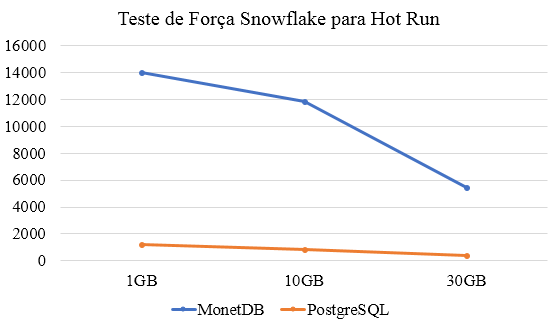
\includegraphics[width=7.2cm]{power_snow_hot}\label{fig:power_snow_hot}}
        \subfigure[]{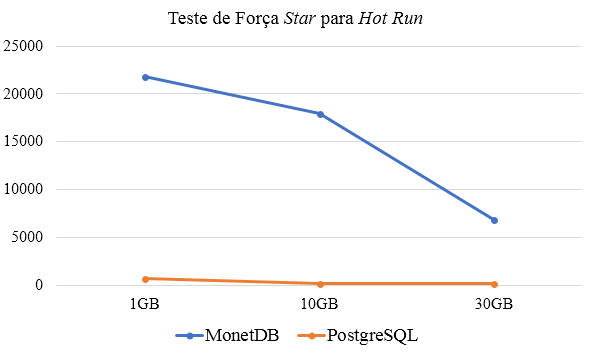
\includegraphics[width=7.2cm]{power_star_hot}\label{fig:power_star_hot}}
        \caption{Gráficos de força entre ambientes sob \textit{hot run}}
        \label{fig:power_hot}
\end{figure*}

Pelo gráfico das Figuras \ref{fig:qph_snow_hot} e \ref{fig:qph_star_hot} percebe-se que o MonetDB continua melhor que o PostgreSQL, conforme os ganhos apresentados na Tabela \ref{tab:ganho_monet_psql_hot}, e agora seus valores também são superiores aos calculados no desempenho final considerando a \textit{cold run}. Ainda, analisando os ambientes sob cada SGBD pelos gráficos das Figuras \ref{fig:qph_monet_hot} e \ref{fig:qph_psql_hot} nota-se pela segunda que o PostgreSQL continua tendo desempenho melhor no ambiente normalizado ao denormalizado, com ganhos de \textbf{40\%, 70\%} e \textbf{53\%} enquanto que a primeira mostra que agora o MonetDB possui valores superiores em todas as bases para o ambiente denormalizado, com ganhos de \textbf{54\%, 63\%} e \textbf{63\%}.

\begin{figure*}[htpb]
        \centering
        \subfigure[]{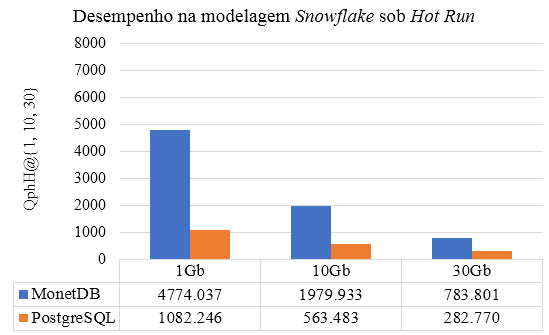
\includegraphics[width=7.2cm]{qph_snow_hot}\label{fig:qph_snow_hot}}
        \subfigure[]{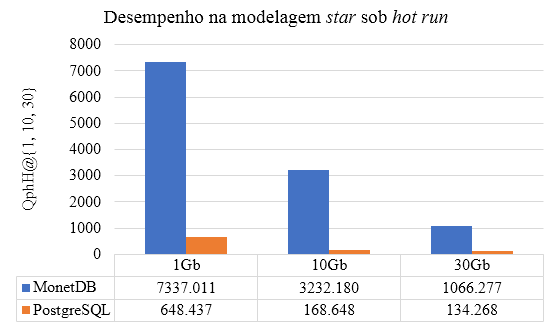
\includegraphics[width=7.2cm]{qph_star_hot}\label{fig:qph_star_hot}}
        \caption{Gráficos de desempenho entre ambientes sob \textit{hot run}}
        \label{fig:qph_model_hot}
\end{figure*}

\begin{table}[htpb]
        \centering
        \caption{Porcentagem de ganho de desempenho do MonetDB em relação ao PostgreSQL sob \textit{hot run}}
        \label{tab:ganho_monet_psql_hot}
        \begin{tabular}{|c|c|c|c|}
        \hline
        \multirow{2}{*}{\textbf{Ambiente}} & \multicolumn{3}{c|}{\textbf{Base de Dados (GB)}} \\ \cline{2-4} 
        & \textbf{1}     & \textbf{10}    & \textbf{30}    \\ \hline
        \textit{Snowflake}                 & 341\%          & 251\%          & 177\%          \\ \hline
        \textit{Star}                      & 1031\%         & 1817\%         & 694\%          \\ \hline
        \end{tabular}
\end{table}
    
\begin{figure*}[t]
        \centering
        \subfigure[]{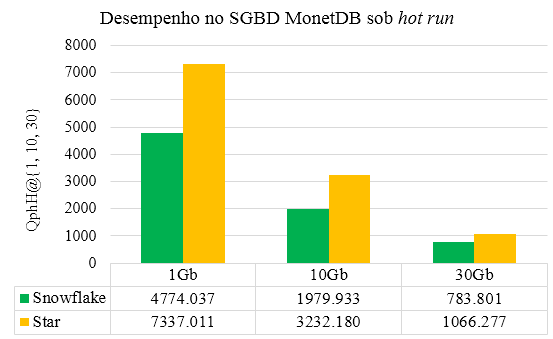
\includegraphics[width=7.2cm]{qph_monet_hot}\label{fig:qph_monet_hot}}
        \subfigure[]{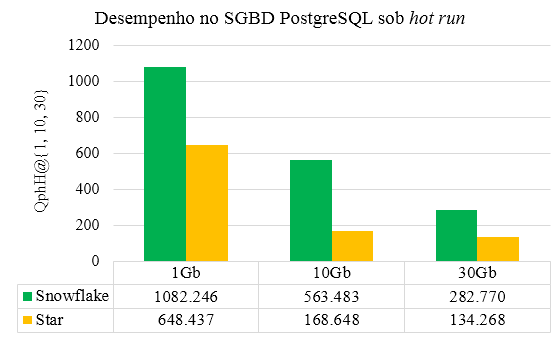
\includegraphics[width=7.2cm]{qph_psql_hot}\label{fig:qph_psql_hot}}
        \caption{Gráficos de desempenho entre SGBD sob \textit{hot run}}
        \label{fig:qph_sgbd_hot}
\end{figure*}

Os valores do SGBD PostgreSQL não tiveram mudanças drásticas se comparadas as execuções \textit{cold} e \textit{hot} das bases de dados de 10GB e 30GB -- inclusive nesta sob a modelagem normalizada o desempenho em \textit{cold run} foi melhor que em \textit{hot run}. A Tabela \ref{tab:ganho_postgresql_cold_hot} mostra a porcentagem de ganho e perdas entre os valores obtidos na terceira execução em relação à primeira execução para o PostgreSQL. Entretanto, os valores do MonetDB se alteraram de forma que houve impacto no resultado final tanto do teste de força como no cálculo final de \textit{benchmark}, como mostram os ganhos da \textit{hot run} em relação à \textit{cold run} na Tabela \ref{tab:ganho_monet_cold_hot}.

\begin{table}[htpb]
        \centering
        \caption{Porcentagem de ganho e perda de desempenho do PostgreSQL da \textit{hot run} em relação à \textit{cold run}}
        \label{tab:ganho_postgresql_cold_hot}
        \begin{tabular}{|c|c|c|c|}
        \hline
        \multirow{2}{*}{\textbf{Ambiente}} & \multicolumn{3}{c|}{\textbf{Base de Dados (GB)}} \\ \cline{2-4} 
        & \textbf{1}     & \textbf{10}    & \textbf{30}    \\ \hline
        \textit{Snowflake}                 & 10\%           & 6\%            & -1\%           \\ \hline
        \textit{Star}                      & 13\%           & 4\%            & 1\%            \\ \hline
        \end{tabular}
\end{table}

\begin{table}[htpb]
        \centering
        \caption{Porcentagem de ganho de desempenho do MonetDB da \textit{hot run} em relação à \textit{cold run}}
        \label{tab:ganho_monet_cold_hot}
        \begin{tabular}{|c|c|c|c|}
        \hline
        \multirow{2}{*}{\textbf{Ambiente}} & \multicolumn{3}{c|}{\textbf{Base de Dados (GB)}} \\ \cline{2-4} 
        & \textbf{1}     & \textbf{10}    & \textbf{30}    \\ \hline
        \textit{Snowflake}                 & 57\%           & 44\%           & 35\%           \\ \hline
        \textit{Star}                      & 74\%           & 58\%           & 54\%           \\ \hline
        \end{tabular}
\end{table}

De acordo com a página oficial do MonetDB \cite{monetdb2017c}, este SGBD se destaca quando dados acessados pelo usuário podem ser mantidos na memória principal do servidor ou quando algumas colunas são solicitadas e são suficientes para manipular uma solicitação, como é o caso do ambiente analítico. Isso explica o porquê das consultas da primeira execução apresentarem desempenho inferior às da terceira execução. Na segunda e na terceira execução alguns dados das consultas já estão em \textit{cache}, assim o SGBD consegue recuperá-los mais rapidamente.

O PostgreSQL, por outro lado, utiliza como \textit{cache} a configuração dos \texttt{shared\_buffers}. Ele corresponde a um vetor de blocos com 8KB, onde o SGBD procura por páginas já alocadas antes de verificar os dados em disco. Para lidar com varreduras sequenciais, são utilizados buffers com valor padrão de 256KB (32 blocos de 8KB) \cite{psqlcache2018r}. Conforme a base de dados aumenta, o ideal é modificar esse valor para que seja possível armazenar mais dados em \textit{cache}, geralmente 25\% da memória total do sistema operacional, porém não mais que 8GB \cite{psql2018conf}. Como esse valor padrão de 256KB não foi alterado, isso explica a variação pequena entre os resultados das bases de dados maiores. O próprio \textit{driver} JDBC possui sua política de \textit{cache} através do \textit{Statement Caching}, sendo opção do desenvolvedor habilitá-la ou não \cite{jdbc2018cache}. Neste trabalho tal política não foi habilitada.

% Statement Cache

Dois exemplos que mostram a estabilidade nos valores alcançados pela \textit{cache} estão na primeira consulta (Q3) e na 11ª (Q14). No cenário de \textit{cold run} a primeira consulta sempre levava mais tempo que as demais e a Q14 demorava excessivamente conforme a base crescia, em detrimento das demais. Considerando este cenário uma justificativa a se utilizar seria a de que as consultas eram demoradas, porém, sob o cenário \textit{hot run} se vê que elas não apresentam o mesmo comportamento, tendo influência da memória \textit{cache}.

\section{Execução com \textit{Drop Cache}}

O último cenário consiste em, levando em consideração que o MonetDB sofre influência da memória \textit{cache}, executar as consultas de força três vezes como no cenário anterior, porém antes da terceira execução efetuar a limpeza na memória \textit{cache} do sistema operacional. A intenção é averiguar se os resultados serão alterados ao mudar o estado da \textit{cache}.

\subsection{Base de Dados de 1GB}

O primeiro detalhe que se nota de acordo com os valores de tempo totais, em segundos, de cada execução de consultas é que a segunda execução é sempre a mais rápida devido a alguns valores já estarem armazenados em \textit{cache}, conforme mostra a Tabela \ref{tab:queries_cache_1}. Após ter limpado parte da \textit{cache}, a terceira execução já torna-se mais lenta que a segunda, porém não mais que a primeira, pois alguns valores ainda podem ter ficado armazenados na memória.

\begin{table}[htpb]
        \centering
        \caption{Tempo total de execução das consultas da 1ª, 2ª e 3ª execução para 1GB}
        \label{tab:queries_cache_1}
        \begin{tabular}{|c|c|c|c|c|}
        \hline
        SGBD       & 1ª Execução & 2ª Execução & 3ª Execução & Ambiente                            \\ \hline
        MonetDB    & 20.842      & 2.811       & 9.973       & \multirow{2}{*}{\textit{Snowflake}} \\ \cline{1-4}
        PostgreSQL & 77.689      & 37.906      & 54.328      &                                     \\ \hline
        MonetDB    & 54.197      & 3.082       & 26.147      & \multirow{2}{*}{\textit{Star}}      \\ \cline{1-4}
        PostgreSQL & 94.184      & 75.135      & 91.649      &                                     \\ \hline
        \end{tabular}
\end{table}

Dentre todas as consultas, a que mais sofreu impacto da oscilação da \textit{cache} foi a primeira. A Tabela \ref{tab:q1_cache_1} mostra os valores para a Q3 de todas as execuções.

\begin{table}[htpb]
        \centering
        \caption{Tempo total de execução da primeira consulta para 1GB}
        \label{tab:q1_cache_1}
        \begin{tabular}{|c|c|c|c|c|}
        \hline
        SGBD       & 1ª Execução & 2ª Execução & 3ª Execução & Ambiente                            \\ \hline
        MonetDB    & 7.758       & 0.228       & 1.034       & \multirow{2}{*}{\textit{Snowflake}} \\ \cline{1-4}
        PostgreSQL & 36.574      & 1.855       & 13.698      &                                     \\ \hline
        MonetDB    & 18.345      & 0.071       & 9.656       & \multirow{2}{*}{\textit{Star}}      \\ \cline{1-4}
        PostgreSQL & 20.054      & 3.038       & 19.919      &                                     \\ \hline
\end{tabular}
\end{table}

As Tabelas \ref{tab:cache_monet_1} e \ref{tab:cache_psql_1} mostram os valores da memória \textit{cache} do sistema operacional durante a execução das consultas para o MonetDB e do PostgreSQL, respectivamente. São mostrados os valores antes da primeira execução, após a primeira e antes da segunda, após a segunda e antes da terceira, após realizar limpeza da \textit{cache} e por fim o valor após finalizar as execuções.

\begin{table}[htpb]
        \centering
        \caption{Valores de \textit{cache} do sistema operacional durante a execução do MonetDB para base de dados de 1GB}
        \label{tab:cache_monet_1}
        \begin{tabular}{c|c|c|c|c|c|}
        \cline{2-6}
        & \textbf{\begin{tabular}[c]{@{}c@{}}Antes da 1ª \\ Execução\end{tabular}} & \textbf{\begin{tabular}[c]{@{}c@{}}Após 1ª \\ Execução\end{tabular}} & \textbf{\begin{tabular}[c]{@{}c@{}}Após 2ª \\ Execução\end{tabular}} & \textbf{\begin{tabular}[c]{@{}c@{}}Após Limpar \\ Cache\end{tabular}} & \textbf{\begin{tabular}[c]{@{}c@{}}Após 3ª \\ Execução\end{tabular}} \\ \hline
        \multicolumn{1}{|c|}{\textit{\textbf{Snowflake}}} & 70029               & 802988                   & 803468                  & 514004     & 791000                 \\ \hline
        \multicolumn{1}{|c|}{\textit{\textbf{Star}}}      & 6940112             & 7689324                  & 7690476                 & 4078724    & 4736752                \\ \hline
        \end{tabular}
\end{table}

\begin{table}[htpb]
        \centering
        \caption{Valores de \textit{cache} do sistema operacional durante a execução do PostgreSQL para base de dados de 1GB}
        \label{tab:cache_psql_1}
        \begin{tabular}{c|c|c|c|c|c|}
        \cline{2-6}
        & \textbf{\begin{tabular}[c]{@{}c@{}}Antes da 1ª \\ Execução\end{tabular}} & \textbf{\begin{tabular}[c]{@{}c@{}}Após 1ª \\ Execução\end{tabular}} & \textbf{\begin{tabular}[c]{@{}c@{}}Após 2ª \\ Execução\end{tabular}} & \textbf{\begin{tabular}[c]{@{}c@{}}Após Limpar \\ Cache\end{tabular}} & \textbf{\begin{tabular}[c]{@{}c@{}}Após 3ª \\ Execução\end{tabular}} \\ \hline
        \multicolumn{1}{|c|}{\textit{\textbf{Snowflake}}} & 10225788	& 11872876	& 11872852	& 511236	& 2133028
        \\ \hline
        \multicolumn{1}{|c|}{\textit{\textbf{Star}}}      & 15037328	& 15480228	& 15481116	& 183448	& 2826952
        \\ \hline
        \end{tabular}
\end{table}

\subsection{Base de Dados de 10GB}

A mesma lógica da base de dados de 1GB segue para a de 10GB, segundo a Tabela \ref{tab:queries_cache_10}. Na execução do PostgreSQL em ambiente \textit{snowflake}, entretanto, houve uma queda no tempo de execução da segunda execução para a terceira, indicando possivelmente menor influência da \textit{cache} neste SGBD.


\begin{table}[htpb]
        \centering
        \caption{Tempo total de execução das consultas da 1ª, 2ª e 3ª execução para 10GB}
        \label{tab:queries_cache_10}
        \begin{tabular}{|c|c|c|c|c|}
        \hline
        SGBD       & 1ª Execução & 2ª Execução & 3ª Execução & Ambiente                            \\ \hline
        MonetDB    & 412.301     & 31.825      & 90.525      & \multirow{2}{*}{\textit{Snowflake}} \\ \cline{1-4}
        PostgreSQL & 950.210     & 750.324     & 744.324     &                                     \\ \hline
        MonetDB    & 398.951     & 50.781      & 294.667     & \multirow{2}{*}{\textit{Star}}      \\ \cline{1-4}
        PostgreSQL & 3042.546    & 2772.970    & 2884.537    &                                     \\ \hline
        \end{tabular}
\end{table}

Nesta base já nota-se de forma acentual a influência da memória na primeira consulta como mostra a Tabela \ref{tab:q1_cache_10}, e consequentemente no resultado final de tempo de execução, podendo ocasionar a mesma inflexão apresentada pela primeira execução dos testes.

\begin{table}[htpb]
        \centering
        \caption{Tempo total de execução da primeira consulta para 10GB}
        \label{tab:q1_cache_10}
        \begin{tabular}{|c|c|c|c|c|}
        \hline
        SGBD       & 1ª Execução & 2ª Execução & 3ª Execução & Ambiente                            \\ \hline
        MonetDB    & 273.352     & 2.460       & 11.734      & \multirow{2}{*}{\textit{Snowflake}} \\ \cline{1-4}
        PostgreSQL & 112.322     & 43.252      & 113.553     &                                     \\ \hline
        MonetDB    & 216.923     & 22.201      & 155.161     & \multirow{2}{*}{\textit{Star}}      \\ \cline{1-4}
        PostgreSQL & 200.664     & 149.393     & 218.902     &                                     \\ \hline
        \end{tabular}
\end{table}

As Tabelas \ref{tab:cache_monet_10} e \ref{tab:cache_psql_10} mostram os valores de \textit{cache} durante as consultas dos SGBD para a base de dados de 10GB.

\begin{table}[htpb]
        \centering
        \caption{Valores de \textit{cache} do sistema operacional durante a execução do MonetDB para base de dados de 10GB}
        \label{tab:cache_monet_10}
        \begin{tabular}{c|c|c|c|c|c|}
        \cline{2-6}
        & \textbf{\begin{tabular}[c]{@{}c@{}}Antes da 1ª \\ Execução\end{tabular}} & \textbf{\begin{tabular}[c]{@{}c@{}}Após 1ª \\ Execução\end{tabular}} & \textbf{\begin{tabular}[c]{@{}c@{}}Após 2ª \\ Execução\end{tabular}} & \textbf{\begin{tabular}[c]{@{}c@{}}Após Limpar \\ Cache\end{tabular}} & \textbf{\begin{tabular}[c]{@{}c@{}}Após 3ª \\ Execução\end{tabular}} \\ \hline
        \multicolumn{1}{|c|}{\textit{\textbf{Snowflake}}} & 791000	& 6366624	& 6387800	& 3685188	& 6213740      \\    \hline
        \multicolumn{1}{|c|}{\textit{\textbf{Star}}}      & 4736752	& 11399260	& 10385332	& 3576824	& 9152120      \\  \hline
        \end{tabular}
\end{table}

\begin{table}[htpb]
        \centering
        \caption{Valores de \textit{cache} do sistema operacional durante a execução do PostgreSQL para base de dados de 10GB}
        \label{tab:cache_psql_10}
        \begin{tabular}{c|c|c|c|c|c|}
        \cline{2-6}
        & \textbf{\begin{tabular}[c]{@{}c@{}}Antes da 1ª \\ Execução\end{tabular}} & \textbf{\begin{tabular}[c]{@{}c@{}}Após 1ª \\ Execução\end{tabular}} & \textbf{\begin{tabular}[c]{@{}c@{}}Após 2ª \\ Execução\end{tabular}} & \textbf{\begin{tabular}[c]{@{}c@{}}Após Limpar \\ Cache\end{tabular}} & \textbf{\begin{tabular}[c]{@{}c@{}}Após 3ª \\ Execução\end{tabular}} \\ \hline
        \multicolumn{1}{|c|}{\textit{\textbf{Snowflake}}} & 2133028	& 12346864	& 12150576	& 182032	& 13263164

        \\ \hline
        \multicolumn{1}{|c|}{\textit{\textbf{Star}}}      & 2826896	& 15058928	& 15153916	& 182628	& 15420316

        \\ \hline
        \end{tabular}
\end{table}

\subsection{Base de Dados de 30GB}

Assim como as anteriores, a Tabela \ref{tab:queries_cache_30} mostra que a terceira execução é afetada pela \textit{cache}, bem como a primeira consulta, cujos valores são mostrados na Tabela \ref{tab:q1_cache_30}.

\begin{table}[htpb]
        \centering
        \caption{Tempo total de execução das consultas da 1ª, 2ª e 3ª execução para 30GB}
        \label{tab:queries_cache_30}
        \begin{tabular}{|c|c|c|c|c|}
        \hline
        SGBD       & 1ª Execução & 2ª Execução & 3ª Execução & Ambiente                            \\ \hline
        MonetDB    & 1062.709    & 495.334     & 688.593     & \multirow{2}{*}{\textit{Snowflake}} \\ \cline{1-4}
        PostgreSQL & 4574.974    & 4433.061    & 4300.868    &                                     \\ \hline
        MonetDB    & 1338.430    & 674.249     & 1243.989    & \multirow{2}{*}{\textit{Star}}      \\ \cline{1-4}
        PostgreSQL & 11128.495   & 10788.900   & 10884.908   &                                     \\ \hline
        \end{tabular}
\end{table}

\begin{table}[htpb]
        \centering
        \caption{Tempo total de execução da primeira consulta para 30GB}
        \label{tab:q1_cache_30}
        \begin{tabular}{|c|c|c|c|c|}
        \hline
        SGBD       & 1ª Execução & 2ª Execução & 3ª Execução & Ambiente                            \\ \hline
        MonetDB    & 487.614     & 122.496     & 322.512     & \multirow{2}{*}{\textit{Snowflake}} \\ \cline{1-4}
        PostgreSQL & 381.837     & 353.038     & 361.421     &                                     \\ \hline
        MonetDB    & 517.566     & 146.583     & 465.564     & \multirow{2}{*}{\textit{Star}}      \\ \cline{1-4}
        PostgreSQL & 586.428     & 570.704     & 571.626     &                                     \\ \hline
        \end{tabular}
\end{table}

As Tabelas \ref{tab:cache_monet_30} e \ref{tab:cache_psql_30} mostram os valores de \textit{cache} durante as consultas dos SGBD para a base de dados de 30GB.

\begin{table}[htpb]
        \centering
        \caption{Valores de \textit{cache} do sistema operacional durante a execução do MonetDB para base de dados de 30GB}
        \label{tab:cache_monet_30}
        \begin{tabular}{c|c|c|c|c|c|}
        \cline{2-6}
        & \textbf{\begin{tabular}[c]{@{}c@{}}Antes da 1ª \\ Execução\end{tabular}} & \textbf{\begin{tabular}[c]{@{}c@{}}Após 1ª \\ Execução\end{tabular}} & \textbf{\begin{tabular}[c]{@{}c@{}}Após 2ª \\ Execução\end{tabular}} & \textbf{\begin{tabular}[c]{@{}c@{}}Após Limpar \\ Cache\end{tabular}} & \textbf{\begin{tabular}[c]{@{}c@{}}Após 3ª \\ Execução\end{tabular}} \\ \hline
        \multicolumn{1}{|c|}{\textit{\textbf{Snowflake}}} & 6214112	& 8495460	& 8866544	& 3892824	& 6940108    \\     \hline
        \multicolumn{1}{|c|}{\textit{\textbf{Star}}}      & 9152508	& 11193612	& 7962648	& 449280	& 10225872     \\     \hline
        \end{tabular}
\end{table}

\begin{table}[htpb]
        \centering
        \caption{Valores de \textit{cache} do sistema operacional durante a execução do PostgreSQL para base de dados de 30GB}
        \label{tab:cache_psql_30}
        \begin{tabular}{c|c|c|c|c|c|}
        \cline{2-6}
        & \textbf{\begin{tabular}[c]{@{}c@{}}Antes da 1ª \\ Execução\end{tabular}} & \textbf{\begin{tabular}[c]{@{}c@{}}Após 1ª \\ Execução\end{tabular}} & \textbf{\begin{tabular}[c]{@{}c@{}}Após 2ª \\ Execução\end{tabular}} & \textbf{\begin{tabular}[c]{@{}c@{}}Após Limpar \\ Cache\end{tabular}} & \textbf{\begin{tabular}[c]{@{}c@{}}Após 3ª \\ Execução\end{tabular}} \\ \hline
        \multicolumn{1}{|c|}{\textit{\textbf{Snowflake}}} & 13844456	& 14718840	& 15093100	& 181636	& 15037352


        \\ \hline
        \multicolumn{1}{|c|}{\textit{\textbf{Star}}}      & 15420712	& 12669240	& 11621556	& 11973800	& 14680412


        \\ \hline
        \end{tabular}
\end{table}

\subsection{Desempenho Geral}

As três subseções anteriores mostraram como a \textit{cache} influencia nos resultados do processamento das consultas, principalmente no SGBD MonetDB. Aplicando o cálculo do teste de força nos valores oriundos da terceira execução é observado a volta da inflexão na base de 10GB, como mostram os gráficos das Figuras \ref{fig:power_snow_cache} e \ref{fig:power_star_cache}.

\begin{figure*}[htpb]
        \centering
        \subfigure[]{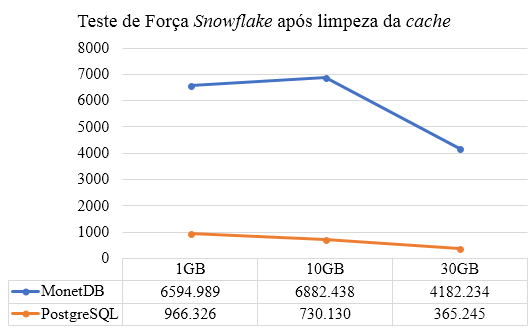
\includegraphics[width=7.2cm]{power_snow_cache}\label{fig:power_snow_cache}}
        \subfigure[]{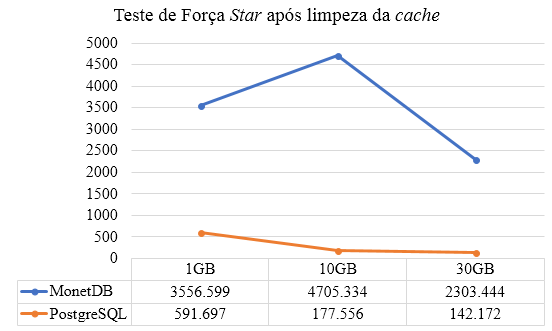
\includegraphics[width=7.2cm]{power_star_cache}\label{fig:power_star_cache}}
        \caption{Gráfico de força entre ambientes sob influência da limpeza de \textit{cache}}
        \label{fig:power_cache}
\end{figure*}

Para averiguar de fato essa influência da limpeza de \textit{cache} na inflexão, o mesmo teste de força foi aplicado nos valores de tempo da segunda execução, que já tinha alguns dados armazenados na memória. Os gráficos das Figuras \ref{fig:power_snow_cache_2} e \ref{fig:power_star_cache_2} ilustram que não ocorreu inflexão na segunda base de dados ao não limpar a \textit{cache}.

\begin{figure*}[htpb]
        \centering
        \subfigure[]{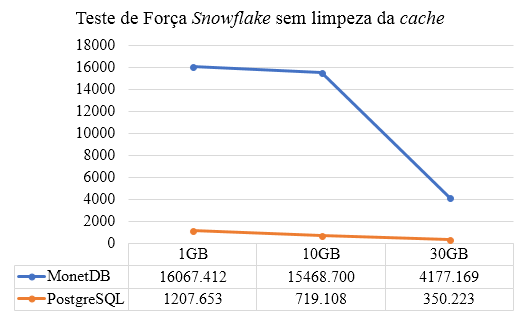
\includegraphics[width=7.2cm]{power_snow_cache_2}\label{fig:power_snow_cache_2}}
        \subfigure[]{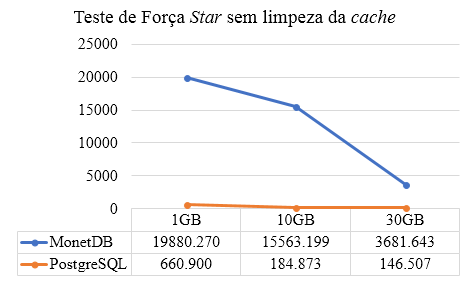
\includegraphics[width=7.2cm]{power_star_cache_2}\label{fig:power_star_cache_2}}
        \caption{Gráficos de força sem limpeza de \textit{cache}}
        \label{fig:power_cache_2}
\end{figure*}

A influência da inflexão pode ser vista na Figura \ref{fig:qph_monet_cache}, que assim como a Figura \ref{fig:qph_monet_cold} não apresenta conclusão acerca da escolha da modelagem para o banco MonetDB. A Figura \ref{fig:qph_psql_cache} mostra os valores finais entre os ambientes no PostgreSQL, e a Figura \ref{fig:qph_model_cache} os gráficos comparando os SGBD dentro de cada ambiente.
    
\begin{figure*}[htpb]
        \centering
        \subfigure[]{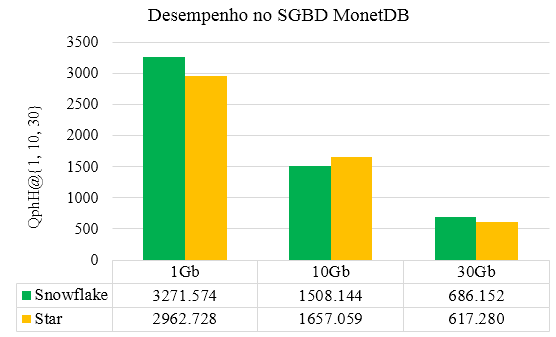
\includegraphics[width=7.2cm]{qph_monet_cache}\label{fig:qph_monet_cache}}
        \subfigure[]{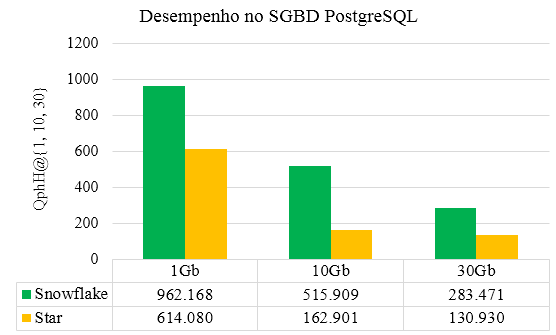
\includegraphics[width=7.2cm]{qph_psql_cache}\label{fig:qph_psql_cache}}
        \caption{Gráficos de desempenho entre SGBD sob influência da limpeza de \textit{cache}}
        \label{fig:qph_sgbd_cache}
\end{figure*}

Considerando a segunda execução, o resultado final de desempenho pode ser visto nos gráficos das Figuras \ref{fig:qph_model_cache_2} e \ref{fig:qph_sgbd_cache_2}. Nelas percebe-se a mesma lógica que as Figuras \ref{fig:qph_model_hot} e \ref{fig:qph_sgbd_hot} apresentam.

\begin{figure*}[htpb]
        \centering
        \subfigure[]{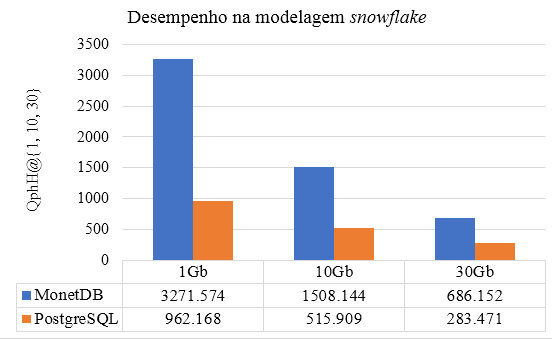
\includegraphics[width=7.2cm]{qph_snow_cache}\label{fig:qph_snow_cache}}
        \subfigure[]{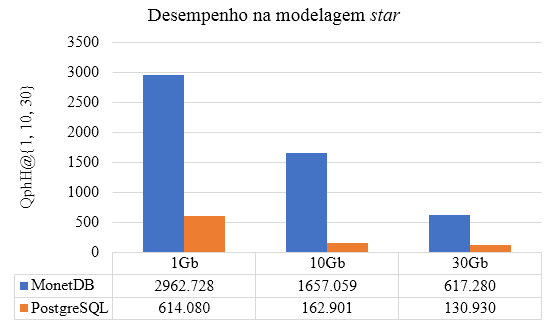
\includegraphics[width=7.2cm]{qph_star_cache}\label{fig:qph_star_cache}}
        \caption{Gráficos de desempenho entre ambientes sob influência da limpeza de \textit{cache}}
        \label{fig:qph_model_cache}
\end{figure*}

\begin{figure*}[t]
        \centering
        \subfigure[]{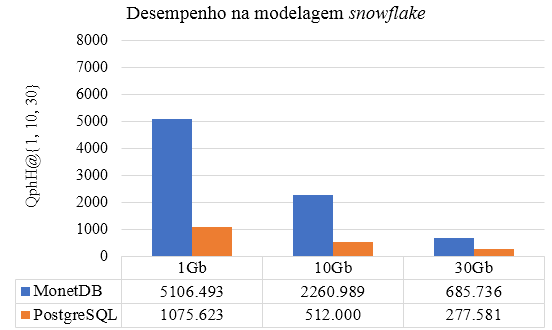
\includegraphics[width=7.2cm]{qph_snow_cache_2}\label{fig:qph_snow_cache_2}}
        \subfigure[]{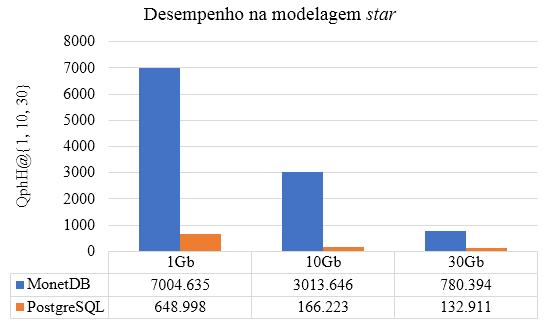
\includegraphics[width=7.2cm]{qph_star_cache_2}\label{fig:qph_star_cache_2}}
        \caption{Gráficos de desempenho entre ambientes sem limpeza de \textit{cache}}
        \label{fig:qph_model_cache_2}
\end{figure*}

\begin{figure*}[htpb]
        \centering
        \subfigure[]{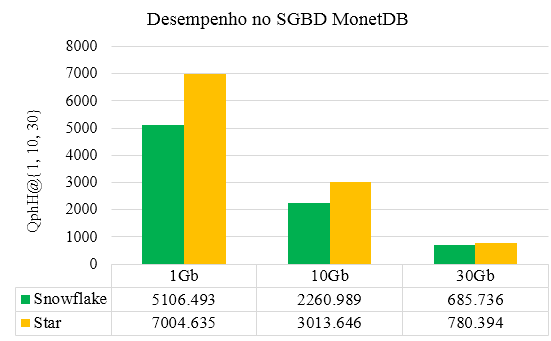
\includegraphics[width=7.2cm]{qph_monet_cache_2}\label{fig:qph_monet_cache_2}}
        \subfigure[]{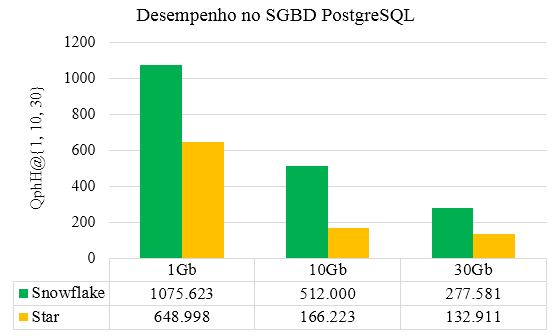
\includegraphics[width=7.2cm]{qph_psql_cache_2}\label{fig:qph_psql_cache_2}}
        \caption{Gráficos de desempenho entre SGBD sem limpeza de \textit{cache}}
        \label{fig:qph_sgbd_cache_2}
\end{figure*}

Entre os trabalhos correlatos, destaca-se o tempo obtido em Rutishauser e Noureldin \cite{rutishauser2012tpc} para o PostgreSQL no ambiente original do TPC-H, \textit{snowflake}, na consulta nas consultas Q8 e Q22, cujos valores são 1.6s e 1s, respectivamente. No cenário \textit{cold run} o PostgreSQL obteve 2.673s e 0.979s, respectivamente. Em \textit{hot run} os resultados foram 2.178s e 0.973s. Entre os demais trabalhos, alguns utilizam SGBD diferentes aos apresentados neste, tornando a comparação dos resultados inviável, mesmo que se utilize o TPC-H. Ainda, mesmo que sejam utilizados o MonetDB e o PostgreSQL, há a aplicação deles em um \textit{benchmark} diferente, o \textit{Star Schema Benchmark}, impossibilitando comparações com o TPC-H devido a implementação da modelagem ser diferente, tanto para o ambiente original quanto para o denormalizado. O próprio TPC apresenta os resultados de \textit{benchmark} para alguns SGBD \cite{tpc2018resultados}, porém só são disponibilizados valores para bases de dados de tamanho superior à 1TB rodando sobre o Microsoft SQL Server \cite{microsoft2018r}.

Considerando o resultado final do \textit{benchmark}, o PostgreSQL se destacou no ambiente normalizado em relação ao denormalizado em todos os cenários por se tratar de um SGBDR, porém, quando comparados os valores de \textit{benchmark} com o MonetDB ele não apresentou destaque sob nenhum cenário, mesmo nos quais o MonetDB mostrou-se instável devido à memória. 

Apesar do destaque do MonetDB, a influencia da memória nele ficou clara ao analisar os valores finais em \textit{cold run} e \textit{hot run}, visto que sob o primeiro cenário ocorreu inflexão fazendo com que o ambiente normalizado tenha resultados melhores que o denormalizado para apenas uma das bases de dados, não trazendo conclusões sobre que ambiente é melhor neste SGBD como gerenciador de DW. No entanto, no segundo cenário pode-se concluir que o melhor ambiente para aplicar o gerenciamento de um DW é o denormalizado, pois todos os valores foram superiores ao normalizado para todas as bases de dados, inclusive se comparar cada valor com o seu correspondente em \textit{cold run}.